\documentclass[ 12pt, xcolor=beamer,table,usenames,dvipsnames, ignorenonframetext, ngerman]{beamer}
\usetheme{Frankfurt}
\usecolortheme{dove}
\usepackage{appendixnumberbeamer}
%\setbeamersize{text margin left=20pt,text margin right=20pt,}
\useoutertheme{miniframes}
\beamertemplatenavigationsymbolsempty 
\setbeamertemplate{mini frames}{}
\setbeamertemplate{itemize item}{\textbullet}

\addtobeamertemplate{navigation symbols}{}{
	\ifnum\insertframenumber>\inserttotalframenumber%
	\relax
	\else%
	\usebeamerfont{footline}%
	\usebeamercolor[fg]{footline}%
	\hspace{1em}%
	\insertframenumber
	\fi%
}
\setbeamercolor{footline}{fg=black}
\setbeamercolor{palette primary}{bg=blue!15,fg=black}
\setbeamercolor{background canvas}{bg=blue!5}
\setbeamercolor{palette secondary}{bg=blue!5}
\setbeamercolor{palette tertiary}{bg=blue!5}
\setbeamercolor{palette quaternary}{bg=blue!5}
\usepackage{soul}
\makeatletter
\let\HL\hl
\renewcommand\hl{%
	\let\set@color\beamerorig@set@color
	\let\reset@color\beamerorig@reset@color
	\HL}

\usepackage{tipa}
\usepackage{tikz}
\usetikzlibrary{shapes.geometric, arrows}
\mode<presentation>

\setbeamercovered{invisible}
\usepackage{multicol}
\usepackage[english]{babel}
\usepackage[latin1]{inputenc}
\usepackage{times}
\usepackage[T1]{fontenc}
\usepackage{ulem}
\usepackage{tipa}
\usepackage{qtree}
\usepackage{phonrule}
\usepackage{graphicx}
\usepackage{apacite}
\usepackage{xcolor}
\setlength\parindent{0pt}
\usepackage{natbib}
\usepackage{tikz}
\usetikzlibrary{arrows.meta}
\usepackage{tcolorbox}
\tcbuselibrary{raster}

\DeclareRobustCommand{\greencheck}{%
	\tikz\fill[scale=0.6, color=ForestGreen]
	(0,.35) -- (.25,0) -- (1,.7) -- (.25,.15) -- cycle;%
}
\title{Extending communication games to more players}
\author{Veronica Boyce}
\begin{document}

\begin{frame}
\maketitle

\end{frame}

\begin{frame}
	THIS IS WHERE WE THANK COLLABORATORS AND FUNDING!
\end{frame}


\begin{frame}{Why study communication?}
	\pause
	Verbal communication is a key method of human interaction.\\ \pause
	% share ideas, teach each other, 
	We communicate and understand more than surface meaning.\\ \pause
	
	Some of this is conventionalized, but some is dynamic. \\
	
%	Verbal communication is a key part of human interaction: we use it to ask for objects, teach
%	facts to others, and express our feelings. We tailor our communication depending on who we are
%	talking to according to our prior interactions with them, what words they know, and what they know
%	about the topic being discussed. This adaptation is dynamic; over the course of a conversation,
%	shared terminology and shorthands naturally arise.
	
\end{frame}

\begin{frame}{Partner-specific adaptation}
	\pause
	How is alignment achieved? 
	
	\pause
	Theoretical angles: \pause
	\begin{itemize} 
		\item Mental modelling (ex. RSA) (Clark \& Wilkes-Gibbs 1986, Goodman \& Frank 2016) \pause
		\item Interactive Alignment Account -- bottom up priming (Garrod \& Pickering 2009) \pause
		\item Audience Design (Yoon \& Brown Schmidt 2019)
	\end{itemize}
\end{frame}

%
\begin{frame}{Clark \& Wilkes-Gibbs 1986}
	
		%\item How do people coordinate in a conversation? 
		%People don't cleanly take turns, don't use full utterances, can do lots of confirmation or repair. 
	%	\item Reference as a microcosm 
		% counter to idealized linguistic or philosophical models, it's messy
	%	\item Tangram reference game has earlier antecedents, but this is foundational to reference coordination, conversational pacts
	%	\item Originates using *this* set of tangrams
		%\item Ordering task, 12 tangrams x 6 rounds, oral communication
	%	\item Timed and transcribed
	%	\item 8 dyads play a reference game
	%	\item Number of words declines over trials steeply between 1 \& 2 and then asymptotes
	%	\item Number of turns also declines
	%	\item Referents become more definite, less hedged
	%	\item Lots of qualitative descriptions
	\pause
	\vspace{-.2cm}
\begin{center}
	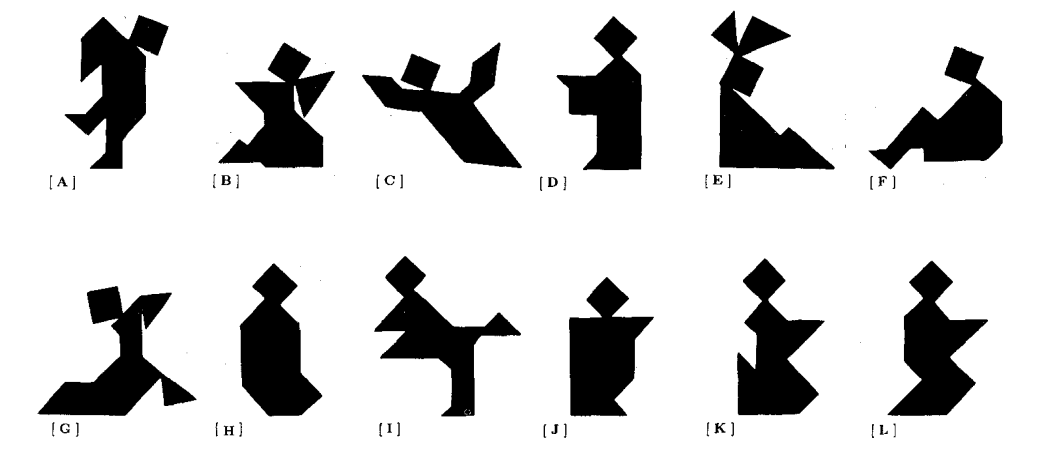
\includegraphics[width=.7\textwidth]{../images/clark_tangrams.png}
	\end{center}
\vspace{-.4cm}
\pause
\begin{small}
\begin{enumerate}
	\setlength{\itemsep}{-2pt}

	\item All right, the next one looks like a person who's ice skating, except, they're sticking two arms out in front. \pause
	\item Um, the next one's the person ice skating that has two arms? \pause
	\item The fourth one is the person ice skating, with two arms. \pause
	\item The next one's the ice skater. \pause
	\item The fourth one's the ice skater. \pause
	\item The ice skater.
	\end{enumerate}
\end{small}
\end{frame}

\begin{frame}{Clark \& Wilkes-Gibbs 1986}
	
	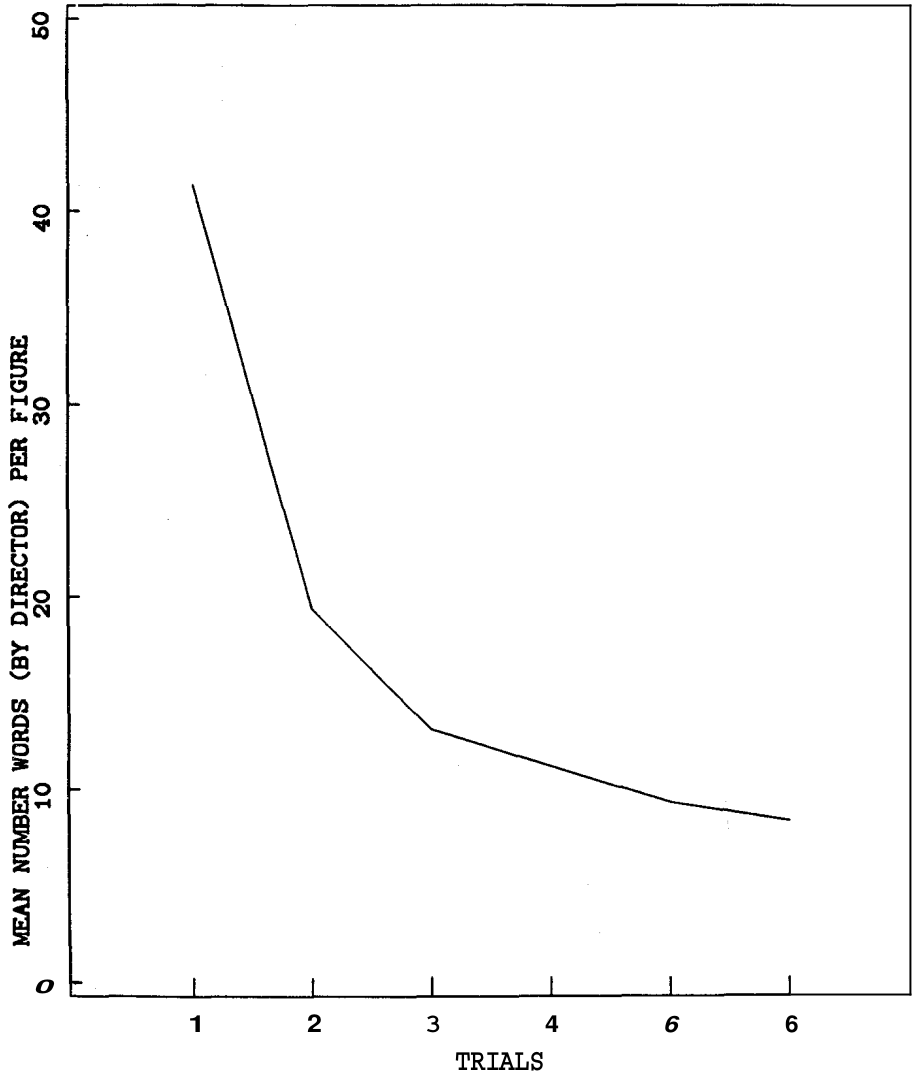
\includegraphics[width=.48\textwidth]{../images/clark_words.png}
		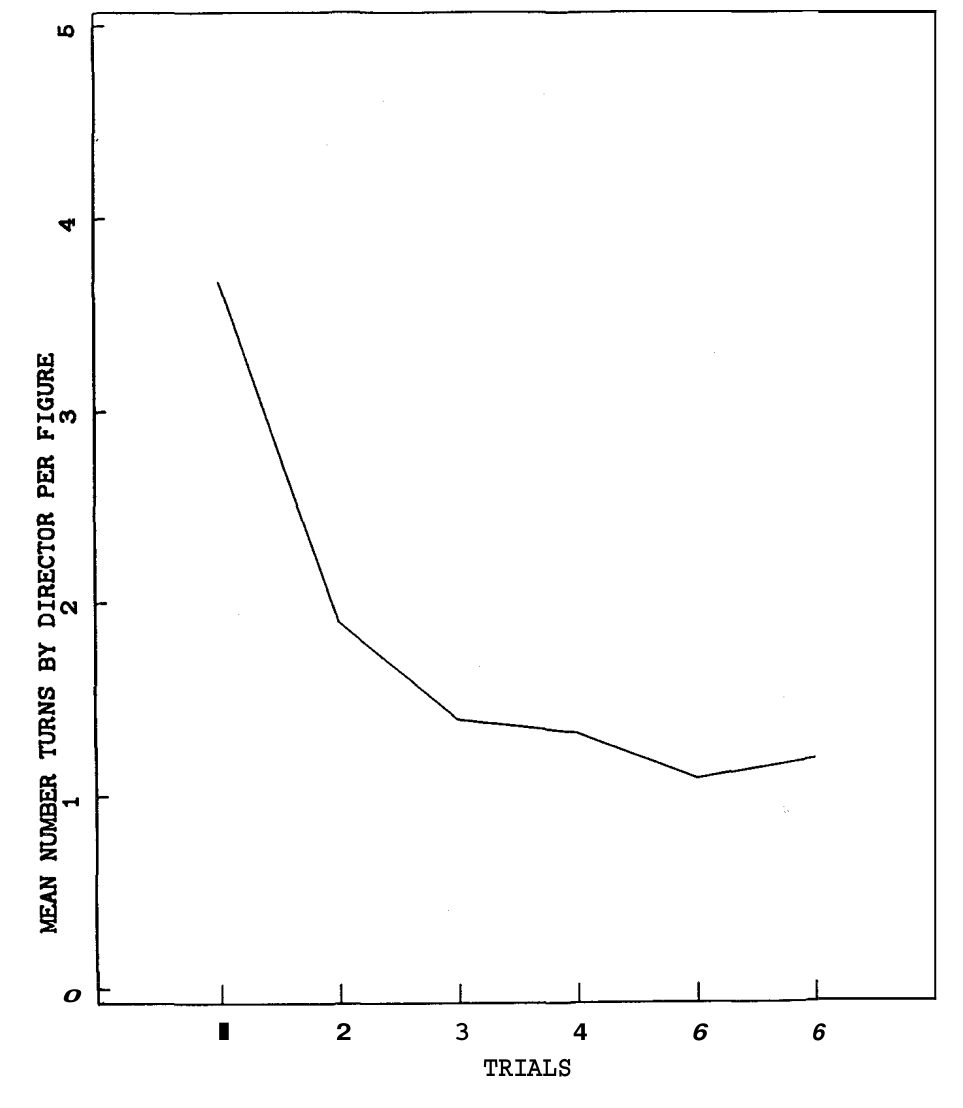
\includegraphics[width=.5\textwidth]{../images/clark_turns.png}	
		
\end{frame}
%
\begin{frame}{Hawkins, Frank, \& Goodman 2020}
Scaling up with web-based experiments
\begin{itemize}
	\item Cued version with feedback on each trial \pause
	\item Message with a chat box \pause
	\item After all exclusions, 83 dyads \pause
\end{itemize}
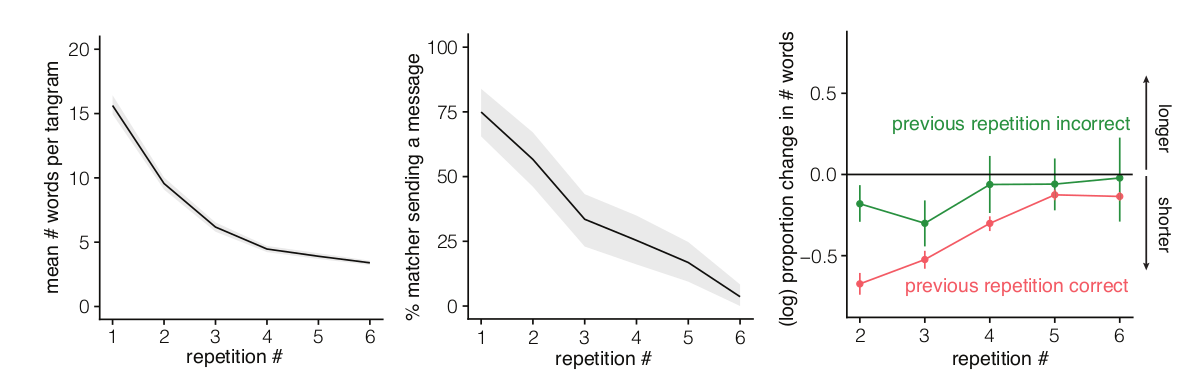
\includegraphics[width=\textwidth]{../images/hawkins_fewer_words.png}
\end{frame}
%
\begin{frame}{Hawkins, Frank, \& Goodman 2020}
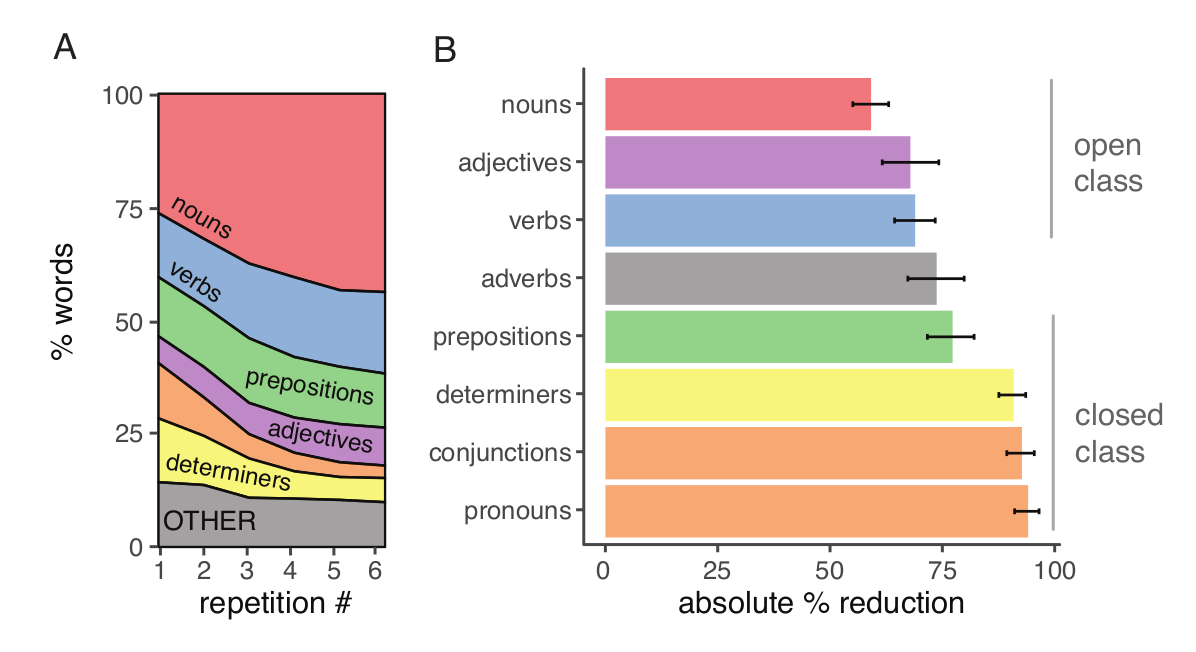
\includegraphics[width=\textwidth]{../images/hawkins_pos.png}
Words tend to drop out in syntactic units
\end{frame}

\begin{frame}{Hawkins, Frank, \& Goodman 2020}
	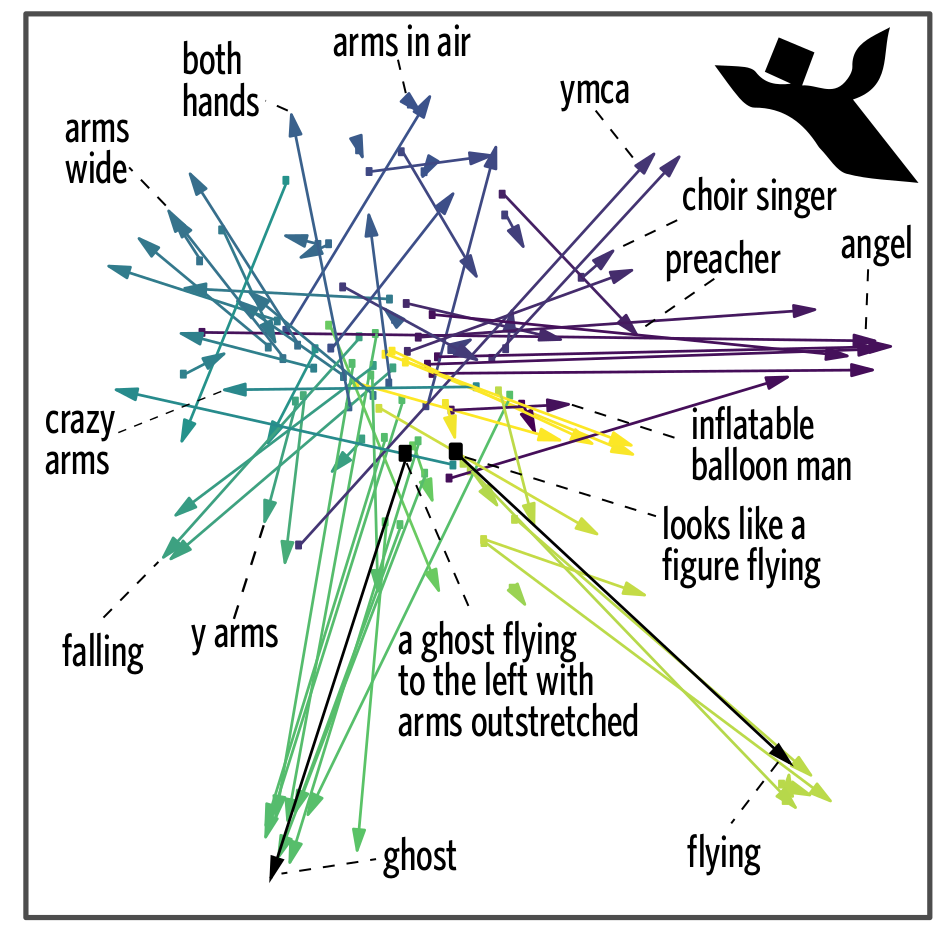
\includegraphics[width=.6\textwidth]{../images/hawkins_semantics.png}
	
	Semantics converge within and diverge between groups
\end{frame}

%
\begin{frame}{FYP}
	What are the dynamics of pact formation between groups? \pause
	 Replicate Hawkins et al to compare groups of 2/3/4 communicators
	\begin{itemize}
		\item Look for differential reduction
		\item 
	\end{itemize} 
Rotate who is the knowledgeable speaker
\begin{itemize}
	\item Chosen for participant experience
	\item Stronger measure of convergence
\end{itemize}

\end{frame}

\begin{frame}{Experiment Framework}
Implemented in Empirica (Almaatouq et al 2020) 
 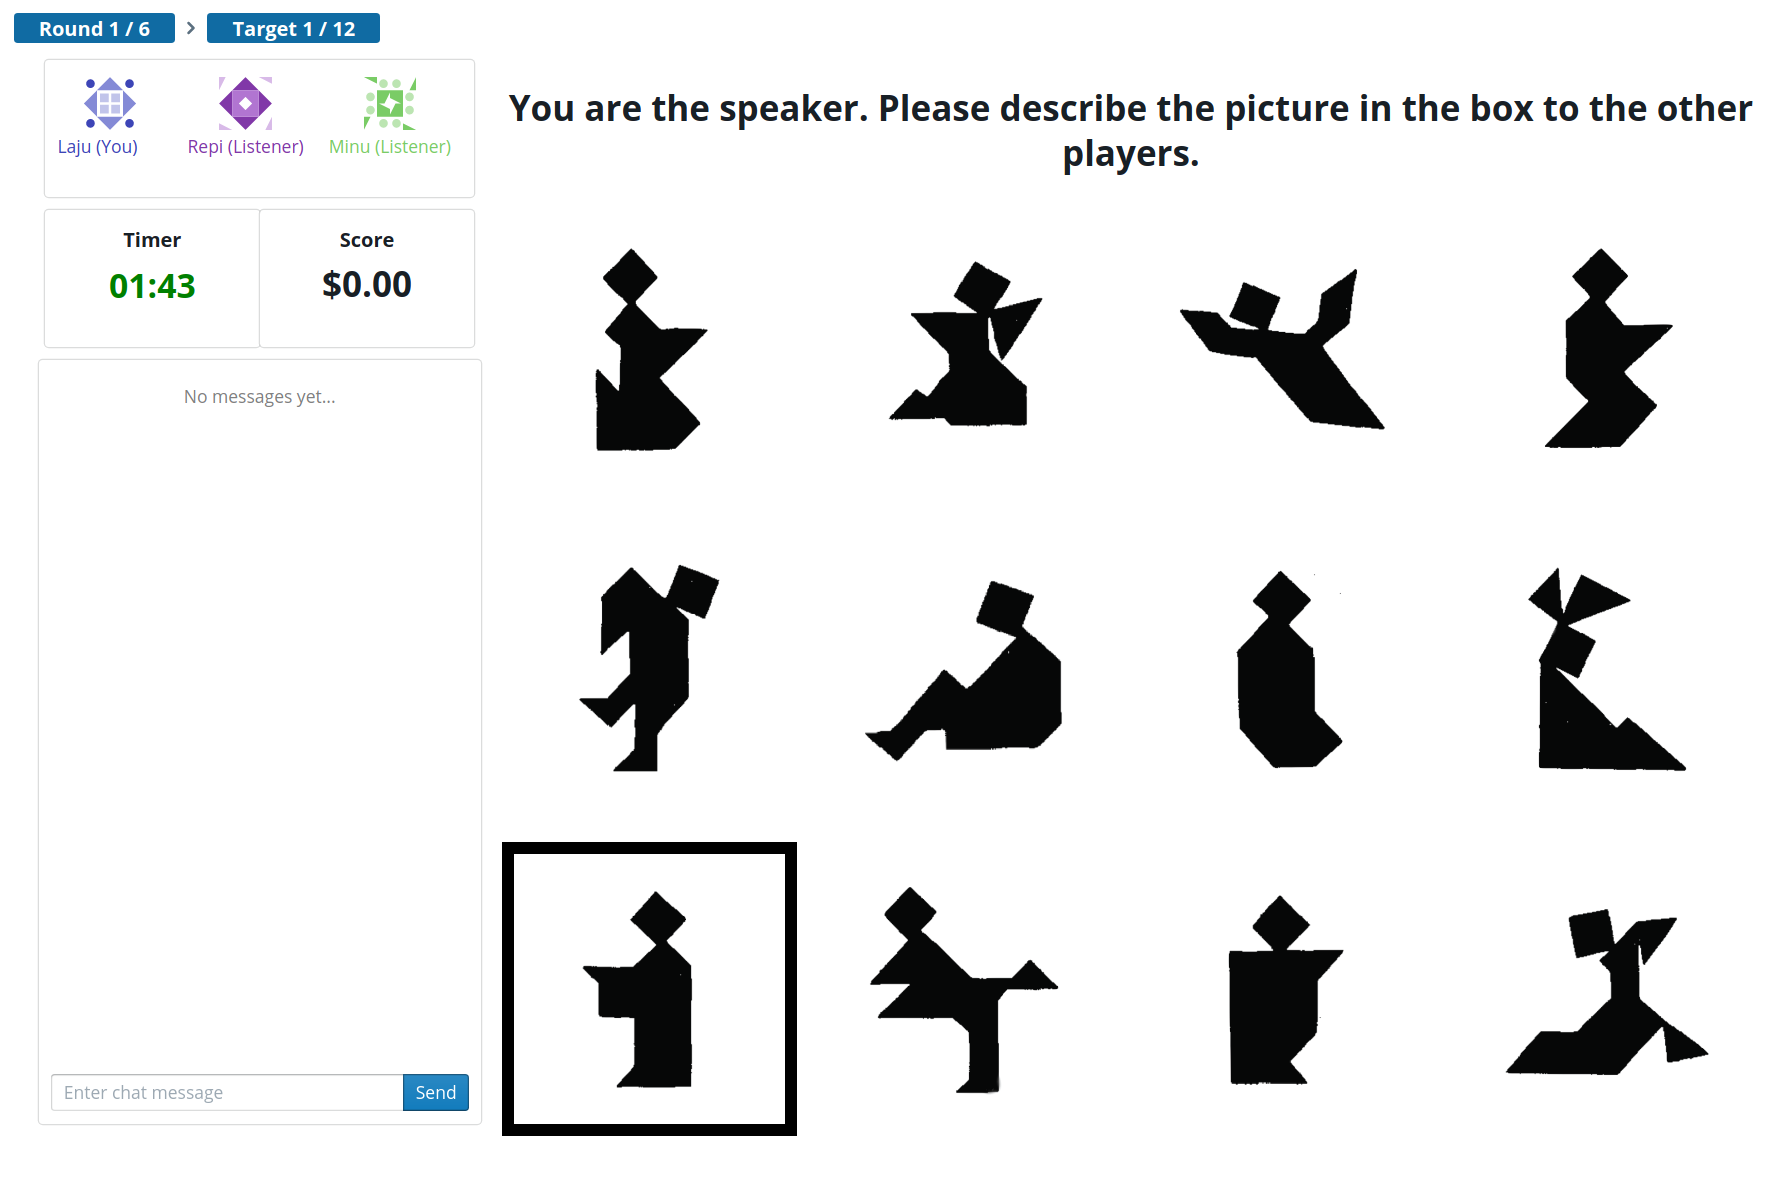
\includegraphics[width=.9\textwidth]{../images/interface.PNG}
\end{frame}

\begin{frame}{Recruitment}
	Goal of 20 complete games in each of 2/3/4 player (60 games, 180 participants)
	Each game has 6 blocks of 12 tangrams
	Actual population:
	\begin{itemize}
		\item YY 4-player games (+ XX partial)
		\item YY 3-player games (+ ZZ partial)
		\item ZZ 2-player games (+ CC partial)
	\end{itemize}
Include all complete blocks
REWARD STRUCTURE!!!!
\end{frame}


\begin{frame}{Results -- Accuracy}
	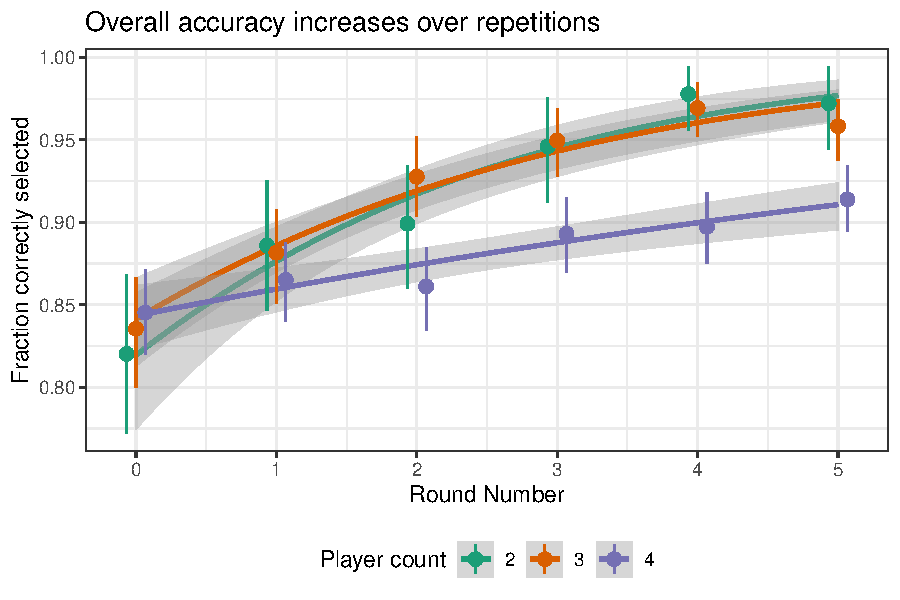
\includegraphics[width=\textwidth]{../images/accuracy.pdf}
	Accuracy is uniformly high, but seems to increase
\end{frame}

\begin{frame}{Results -- Speed}
	
	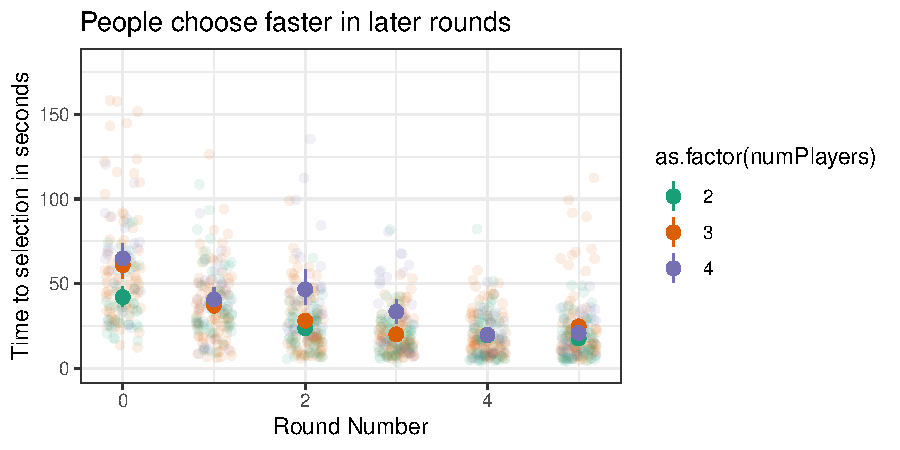
\includegraphics[width=\textwidth]{../images/time.pdf}
	Listeners choose faster in later rounds
	
\end{frame}

\begin{frame}{Reduction}
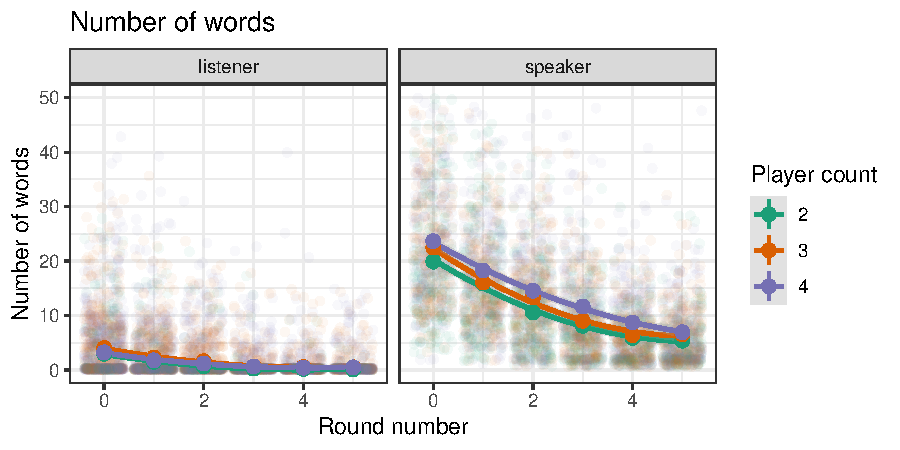
\includegraphics[width=\textwidth]{../images/words.pdf}
OVERALL PICTURE HERE
Plan to remove chit-chat
\end{frame}

\begin{frame}{Reduction}
	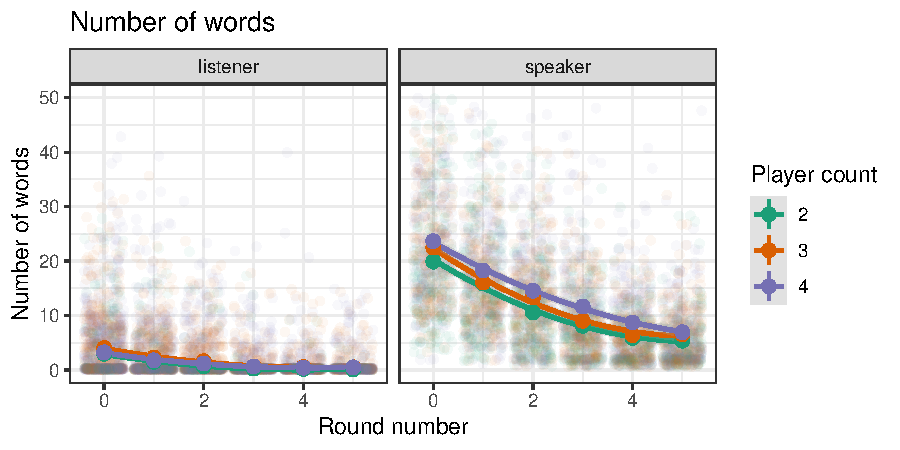
\includegraphics[width=\textwidth]{../images/words.pdf}
Broken out by tangram
\end{frame}

\begin{frame}
	TODO wacky when to reduce charts here
\end{frame}

\begin{frame}
	Future steps:
	- clean up analyses and run models to confirm what we already see
	--> reduce less for more players
	Why? and How?
	--> what are the differences in language
	Semantic analyses -- how do statements change across rounds (and as a product of if they got it right?)
	How do these trajectories change for number of players?
	Check for Listener-Listener interactions
\end{frame}


\begin{frame}{Possible future directions}
	Want to understand how references are formed more generally
	\begin{itemize}
	\item Very flexible framework \pause
	\item Quantify how far the key findings generalize \pause
	\item Explore mechanisms and untangle theories \pause
\end{itemize}
 Possible knobs:\pause
\begin{itemize}

	\item Target images \pause
	\item Curriculum learning
\end{itemize}

\end{frame}


\begin{frame}{Bigger picture}
	\begin{itemize}
		\item Connections to teaching \pause
		\item Tie this into modelling work \pause
		\item Dataset for training AI agents for conversation
	\end{itemize}
\end{frame}

\begin{frame}{Comments, Questions?}
	Looking for feedback on
	\smallskip
	\begin{itemize}
	\item What analyses would be interesting?
	\item What's the next study?
	\end{itemize}
\end{frame}

\appendix

\begin{frame}{Yoon \& Brown-Schmidt 2019}
Speaker talks to multiple matchers of different knowledge levels\\


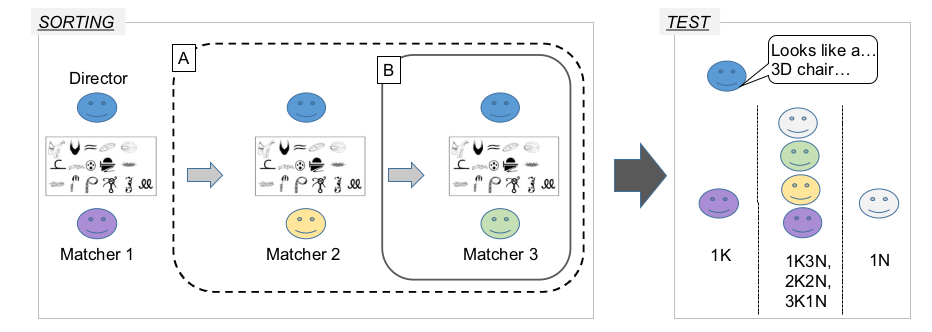
\includegraphics[width=\textwidth]{../images/yoon_diagram.png}

Examine speaker's utterances for length, elaborations, disfluencies
%length, elaboration, disfluencies
\end{frame}

\end{document}

